\documentclass[a4paper]{article}

\usepackage{INTERSPEECH2018}
\usepackage[british,UKenglish]{babel}

\title{An LSTM Language Model for Wakirike}
\name{Iyalla John Alamina$^1$, David Wilson$^1$, Andrew Crampton$^1$}
%The maximum number of authors in the author list is twenty. If the number of contributing authors is more than twenty, they should be listed in a footnote or in acknowledgement section, as appropriate.
\address{
  $^1$University of Huddersfield, United Kingdom}
\email{john.alamina@hud.ac.uk, d.r.wilson@hud.ac.uk, a.crampton@hud.ac.uk}

\begin{document}

\maketitle
% 
\begin{abstract}
In this paper, a character-based Recurrent Neural Network (RNN) language model is implemented for the Wakirike language as a strategy to address the under-resourced nature of the language for Automatic Speech Recognition (ASR) speech processing.  In this work, a comparable Long Short Term Memory (LSTM) deep RNN Language model is prescribed as a step towards faster and resource affordable ASR systems.  

The Language model implemented in this article while having a small text corpus size was found to be potentially powerful enough to be comparable with the state of the art language models yielding a better relative perplexity score of 2.6 when compared to the score of 3.2 on the n-gram model with smoothing.
\end{abstract}
\noindent\textbf{Index Terms}: Recurrent Neural Networks, Long Short-Term Memory, Deep Neural Networks, Speech Recognition, Language Model, RNN, DNN, LSTM.

\section{Introduction}

In recent times there has been a significant amount of effort in the Speech recognition research community to tackle the pragmatic reality of scarcity of speech data when building speech processing systems.  Comparing to a child learning a language between the ages of 2 to 5, a child is able to grasp the fundamentals of a language by being exposed to approximately 4000 hours of speech between these ages \cite{versteegh2015zero}.  For automatic speech recognition systems to obtain reasonable results would require between 200 to 2000 hours of aligned speech data, that is, data having both text and speech\cite{hannun2014deep}.  Low resource speech recognition is therefore significant for two reasons. The first is the ability to build and reproduce speech recognition/speech processing systems for a variety of uses and languages; the second is for the purpose of optimising resources within the various domains being used by these speech systems.

Broadly speaking a language can be described as low resourced, resource-poor or low-data \cite{besacier2014automatic} given that one or more of the following components is either limited or absent: electronic resources, an orthographic writing system, transcribed and recorded speech data, dictionary and other linguistic resources such as a phonetic dictionary and other related linguistic descriptions. This paper focuses on Wakirike language which is especially deficient in transcribed speech data.  There exists a limited language dictionary for Wakirike language from which a phonetic dictionary can be derived.

One key aspect of speech recognition systems which all modern state-of-the-art Automatic Speech Recognition (ASR) systems rely on is the language model.  The language model of an ASR system is a semantic bridge for the ASR system to form meaningful utterances from words and syllables detected or recognised.  Language models have many uses in natural language applications such as word prediction, spell checking, optical character recognition etc.  The model described in this paper builds a character-based recurrent neural network which is quite a powerful model and yet is modestly resourced.  Traditionally, language models derive language-semantic information by counting word occurrences and word-pair occurrences \cite{allen1995natural,jelinek1976continuous}. The recurrent neural network on the other hand builds an internal representation of the language based on long-term conditional relationships between successive characters in the training corpus \cite{mikolov2011empirical}.   From a semantic stance, it is more logical to create a word-based language model than a character based language model.  However in a resource lacking scenario, there are many gains from using a character-based model when compared to a word-based model.  This is due to the fact that the data preparation process requires processing of the raw corpus alone without having a separate language vocabulary.  In addition, the character based model does not suffer from out-of-vocabulary words because the character-set is a well defined and fixed set while the word vocabulary set is potentially infinite as new words are coined within various language-modifying circumstances.

The results showed that for a small corpus of about one hundred thousand words, a comparable language model could be built. The next section surveys various language model techniques used in Automatic Speech Recognition systems and in the section afterwards is a description of the recurrent neural network (RNN) technique used in this paper as well as the corpus used to create the language model.  The fourth section is a presentation of the results of the experiments performed and an evaluation and conclusion presented in the last section.


\section{Literature Review}

Statistical speech recognition is made possible by breaking down an intractable probability distribution of words given acoustic data by applying Bayesian logic. The result of this simplification is a tractable two step procedure where the acoustic probability distribution is multiplied by the probability of words known as a language model \cite{gales2007}.  The probability distribution of words or language model has been traditionally obtained by counting words and using the Markov chain simplification within a Maximum Likelihood Estimation framework.  Best performance of this framework known as the n-gram model is achieved using various smoothing techniques \cite{chen1996empirical}.

As computing power and availability of big data became ubiquitous, the applications of neural network to more areas of research have been seen to be an alternative approach to conventional methods of machine learning and especially pattern recognition. Because the statistical language model attempts to determine the pattern of a language through conditional probabilities between words, it is also possible to achieve the same using deep neural networks. 

In 2003, Bengio et.al. \cite{bengio2003neural} proposed a language model based on neural multi-layer perceptrons (MLPs). These MLP language models resort to a distributed representation of all the words in the vocabulary such that the probability function of the word sequences is expressed in terms of these word-level vector representations. The result of the MLP-based language models was found to be, in cases for models with large parameters, performing better than the traditional n-gram models.

Improvements over the MLPs still using neural networks over the next decade include works of \cite{mikolov2011empirical,sutskever2014sequence,luong2013better}, involved the utilisation of deep neural networks for estimating word probabilities in a language model.  While a Multi-Layer Perceptron consists of a single hidden layer in addition to the input and output layers, a deep network in addition to having several hidden layers are characterised by complex structures that render the architecture beyond the basic feed forward nature where data flows from input to output hence in the RNN architecture we have some feedback neurons as well.  Furthermore, the probability distributions in these deep neural networks were either based upon word or sub-word models this time having representations which also conveyed some level of syntactic or morphological weights to aid in establishing word relationships.  These learned weights are referred to as token or unit embeddings.

For the neural network implementations so far seen, a large amount of data is required due to the nature of words to have large vocabularies, even for medium-scale speech recognition applications.  Yoon Kim et. al. \cite{kim2016character} on the other hand took a different approach to language modelling taking advantage of the long-term sequence memory of long-short-term memory cell recurrent neural network (LSTM-RNN) to rather model a language based on characters rather than on words.  This greatly reduced the number of parameters involved and therefore the complexity of implementation.  This method is particularly of interest to this article and forms the basis of the implementation described in this article due to the low resource constraints imposed when using a character-level language model.

Other low resource language modelling strategies employed for the purpose of speech recognition was demonstrated by \cite{xu2013cross}.  The language model developed in that work was based on phrase-level linguistic mapping from a high resource language to a low resource language using a probabilistic model implemented using a weighted finite state transducer (WFST). This method uses WFST rather than a neural network due to scarcity of training data required to develop a neural network. However, it did not gain from the high nonlinearity ability of a neural network model to discover hidden patterns in data, being a shallower machine learning architecture.

The method employed in this article uses a character-based Neural network language model that employs an LSTM network similar to that of \cite{kim2016character} on the Okrika language which is a low resource language bearing in mind that the character level network will reduce the number of parameters required for training just enough to develop a working language model for the purpose of speech recognition.  The description of the data and procedure used to develop the language model is discussed in the next section. 

\section{The LSTM Cell Recurrent Neural Network}


Neural networks have become increasingly popular due to their ability to model non-linear system dynamics. Since their inception, there have been many modifications made to the original design of having linear affine transformations terminated with a nonlinear functions as the means to capture both linear and non-linear features of the target system. In particular, one of such neural network  modifications, namely the recurrent neural network, has been shown to overcome the limitation of varying lengths in the inputs and outputs of the classic feed-forward neural network.  In addition the RNN is not only able to learn non-linear features of a system but has also been shown to be effective at capturing the patterns in sequential data.

This work draws upon the premise that the grammar of a language is expressed in the character sequence pattern which is ultimately expressed in words and therefore the abstract grammar rules can be extracted and learned by a character-based RNN neural network.  A special implementation of the RNN called the Long Short Term Memory (LSTM) has been designed to capture patterns over particularly long sequences of data and thus is an ideal candidate for generating character sequences while preserving syntactic language rules learned from the training data.

The internal structure and working  of the LSTM cell is documented by its creators in \cite{sak2014long}. The ability to recall information over extended sequences results from the internal gated structure which performs a series of element wise multiplications on the inputs and internal state of the LSTM cell at each time step.  In addition to the output neurons which in this text we refer to as the write gate and denote as the current cell state, $\mathbf{c}_t$, three additional gates (comprising a neural network sub-layer) located within the LSTM cell are the input gate, the forget gate and the output gate.  Together with the initial current state cell these gates along with the current-state cell itself enable the LSTM cell architecture to store information, forward information, delete information and receive information.  Generally however, the LSTM cell looks like a regular feed-forward network having a set of neurons capped with a nonlinear function.  The recurrent nature of the network arises, however due to the fact that the internal state of the RNN cell is rerouted back as an input to the RNN cell or input to the next cell in the time-series give rise to sequence memory within the LSTM architecture. Mathematically, these gates are formulated as follows:

% 
\begin{equation}
\mathbf{i}_t=\sigma(\mathbf{W}^{(xi)}\mathbf{x}_t+\mathbf{W}^{(hi)}\mathbf{h}_{t-1}+\mathbf{W}^{(ci)}\mathbf{c}_{t-1}+\mathbf{b}^{(i)})
  \label{eq1}
\end{equation}
%
%
\begin{equation}
\mathbf{f}_t=\sigma(\mathbf{W}^{(xf)}\mathbf{x}_t+\mathbf{W}^{(hf)}\mathbf{h}_{t-1}+\mathbf{W}^{(cf)}\mathbf{c}_{t-1}+\mathbf{b}^{(f)})
\label{eq2}
\end{equation}
%
%
\begin{equation}
\mathbf{c}_t=\mathbf{f}_t\bullet\mathbf{c}_{t- 1}+\mathbf{i}_t\bullet\tanh(\mathbf{W}^{(xc)}\mathbf{x}_t+\mathbf{W}^{(hc)}\mathbf{h}_{t-1}+\mathbf{b}^{(c)})
\label{eq3}
\end{equation}
%
%
\begin{equation}
\mathbf{o}_t=\sigma(\mathbf{W}^{(xo)}\mathbf{x}_t+\mathbf{W}^{(ho)}\mathbf{h}_{t-1}+\mathbf{W}^{(co)}\mathbf{c}_{t-1}+\mathbf{b}^{(o)})
\label{eq4}
\end{equation}
%
%
\begin{equation}
\mathbf{h}_t=\mathbf{o}_t\bullet\tanh{(\mathbf{c}_t)} 
\label{eq5}
\end{equation}
%


\begin{figure}
\centering
  % Requires \usepackage{graphicx}
  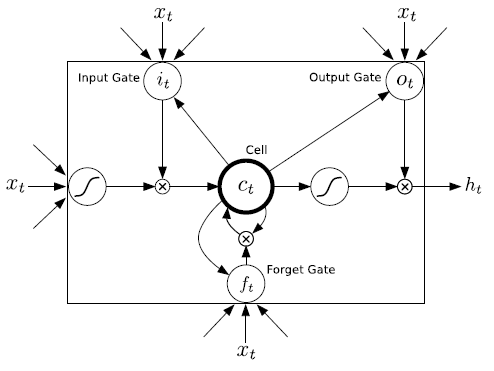
\includegraphics[width=7cm]{lstmcell}\\
  \caption{LSTM Cell \cite{graves2013hybrid}}\label{fig1:lstmcell}
\end{figure}

The gates in the above formula are illustrated in Figure ~\ref{fig1:lstmcell}.  $\mathbf{i}_t$ represents the input gate, $\mathbf{f}_t$ is the forget gate and $\mathbf{o}_t$ represents the output gate.  At each of these gates therefore, the inputs consisting of hidden states in addition to the regular inputs are multiplied by a set of weights and passed through a soft-max function. These weights during training learn whether the gate will, during inference, open or not. In summary, the input gate tells the LSTM not whether or not to receive new information, the forget gate determines whether the current information it already has from the previous step should be kept or dropped and the output gate determines what should be forwarded to the next LSTM cell.  Note also that the LSTM has two sigmoid (tanh) activation functions utilised at the input and output of the current cell $\mathbf{c}_t$.

\subsection{Dataset Preparation}
The Wakirike new testament bible served as the source of data for the deep neural network training.  As there wasn't a soft or on-line copy of the Wakirike new testament bible readily available for use, the four gospels of the Wakirike new testament bible were quickly typed and duplicated once giving a complete corpus word size of about 165,180 words.  This gracefully yielded a character count of about 1,113,820 characters void of punctuation characters. The dataset was then divided 1 in 10 parts for testing and the remaining 9 parts were used for training.

During data preparation, the dataset was first striped off all punctuation marks such that only characters and spaces are selected.  Next, each character in the dataset was substituted with its equivalent Unicode numeric representation. Finally the numeric values were one-hot encoded deriving a sparse array of values having unique indexes set to one for each unique Unicode value and zero every where else. One-hot encoded array therefore, for each character input.

\subsection{LSTM Training}

In order to optimise performance of the network a modified LSTM cell known as the Gated Recurrent Unit (GRU) replaced the LSTM in the neural network model.  These GRUs have been shown to give similar performance to regular LSTMs with a lighter system resource consumption foot print \cite{cho2014learning}. The internal network size of the GRU was 256 nodes and the number of GRUs representing each time step in the recurrent input sequence was 30 GRUs; one GRU per time step. In addition, each unrolled sequence was layered 3 times.  Therefore the unrolled 30-GRU-sequence long network was also 3-layers deep. Due to the multi-layered high-dimensional depth of this neural network, there was a tendency for the network to over fit the data, hence, a small learning rate of 0.001 was used. To further reduce the risk of over fitting the popular and effective dropout method for regularising deep neural networks kept at 80\% of activations while deactivating the rest.

\subsection{LSTM Output Language Generation}
Once training of the neural network as described above is completed after several epochs or training cycles to an acceptable margin of error. It is possible to seed the network with an input character and the model samples from the top-N most likely candidates.  We thus have instructed the language model developed to immanently construct its own sentences.  The output language should therefore be intelligible similar to the training data. 

In this work, the output language generated was used to generate a corpus that measured the perplexity and compared the result with the perplexity based on an n-gram model applied to the original training data.  The results discussed below showed that the LSTM model generated a superior model compared to the n-gram model that better matched the training data.

\section{Discussion}
For the Wakirike LSTM language model used in this work, a corpus of the Wakirike language having a word size of 165,180 words of the New Testament Gospels in Wakirike language was utilised. The vocabulary of this corpus had a word size of approximately 5,000 words. The corpus generated by the LSTM-RNN character sequence model from the original corpus produced a word size of 118,000 words. However the vocabulary of the output LSTM corpus almost doubled to the tune of about 9000 words. 

The result of the training of the Long-short-term-memory (LSTM)-Cell Recurrent Neural Network on low-resourced Wakirike Language gave impressive and intelligible results and showed better results when measured with standard n-gram language models. The results showed that it is indeed possible to use an LSTM on a low resource character sequence corpus to produce an Wakirike language model.

The evaluation of the LSTM language model of the Wakirike language was performed using a perplexity measurement metric. The Perplexity metric applies the language model to a test dataset and measures how probable the test dataset is. Perplexity is a relative measure given by the formula:

%
\begin{equation}
PP(W)=P(w_1,w_2\dots w_N)^\frac{1}{N}
\label{eq6}
\end{equation}
%
%
\begin{equation}
PP(W)=\sqrt[N]{\prod_{i=1}^N\frac{1}{P(w_i|w_{i-1})}}
\label{eq7}
\end{equation}
%

Where $w_1,\dots,w_N$ are the sequence of words. The language model with the lower relative perplexity score is therefore expected to yield better approximation of the data when applied to unseen data generally.

There was no way however to directly measure perplexity on a character sequence model because perplexity is usually used to evaluate word-based models.  However, this limitation was overcome by performing n-gram analysis on the corpus entirely generated from the LSTM network. The generated n-gram model from the generated corpus is then applied to test data and the perplexity is measured.

Table ~\ref{tab:example} below shows the Results of the Perplexity model of the LSTM Wakirike Language model and an equivalent Trigram Language model with interpolation and Keysner smoothing \cite{chen1996empirical}.
Table 1 below shows the Results of the Perplexity model of the LSTM Wakirike Language model and an equivalent Tri-gram Language model with interpolation and Keysner smoothing \cite{chen1996empirical}.
\begin{table}
  \caption{Perplexity Calculation results}
  \label{tab:example}
\begin{tabular}{lr}
\toprule
Language Model & Perplexity\\
\midrule
LSTM RNN & 2.6\\
3-gram with Keysner Soothing and interpolation & 3.3\\
\bottomrule
\end{tabular}
\end{table}

\section{Conclusion}
There is a strong need to consolidate and optimise the research being carried out in automatic speech recognition.  An exciting aspect of the research is the need to verify methods on different languages not previously exposed to the current ASR methods.  This paper presented an LSTM language model for Wakirike language as a step towards low resource speech recognition.  The LSTM language model, was optimised using a bespoke character-based LSTM model to compensate for the low resource text data seen in Wakirike as a language. At the same time, the LSTM RNN model produced a fine-grained language model as opposed to traditional word-based models or other statistical models and was able to produce acceptable results. Having seen the perplexity measurement that performed better than the statistical language model counterparts, the language model produced in this work can serve as a basis for a more elaborate generative model which can in turn serve as a substrate for generative adversarial techniques. Conversely, generative adversarial techniques \cite{goodfellow2014generative}, which is the subject of a future work, presents a valuable method to tackle the low resource ASR challenge.

\section{Acknowledgements}

The authors would like to thank Andrej Karpathy and Martin Gomer for their character LSTM implementations from which this work was adapted.


\bibliographystyle{IEEEtran}

\bibliography{mybib}

% \begin{thebibliography}{9}
% \bibitem[1]{Davis80-COP}
%   S.\ B.\ Davis and P.\ Mermelstein,
%   ``Comparison of parametric representation for monosyllabic word recognition in continuously spoken sentences,''
%   \textit{IEEE Transactions on Acoustics, Speech and Signal Processing}, vol.~28, no.~4, pp.~357--366, 1980.
% \bibitem[2]{Rabiner89-ATO}
%   L.\ R.\ Rabiner,
%   ``A tutorial on hidden Markov models and selected applications in speech recognition,''
%   \textit{Proceedings of the IEEE}, vol.~77, no.~2, pp.~257-286, 1989.
% \bibitem[3]{Hastie09-TEO}
%   T.\ Hastie, R.\ Tibshirani, and J.\ Friedman,
%   \textit{The Elements of Statistical Learning -- Data Mining, Inference, and Prediction}.
%   New York: Springer, 2009.
% \bibitem[4]{YourName17-XXX}
%   F.\ Lastname1, F.\ Lastname2, and F.\ Lastname3,
%   ``Title of your INTERSPEECH 2018 publication,''
%   in \textit{Interspeech 2018 -- 19\textsuperscript{th} Annual Conference of the International Speech Communication Association, September 2-6, Hyderabad, India Proceedings, Proceedings}, 2018, pp.~100--104.
% \end{thebibliography}

\end{document}
